\chapter{Single Stage Amplifiers}
From the \textit{Microelectronics} textbook here's a diagram on four amplifier types before going into single stage amplifiers.
\begin{figure}[H]
    \centering
    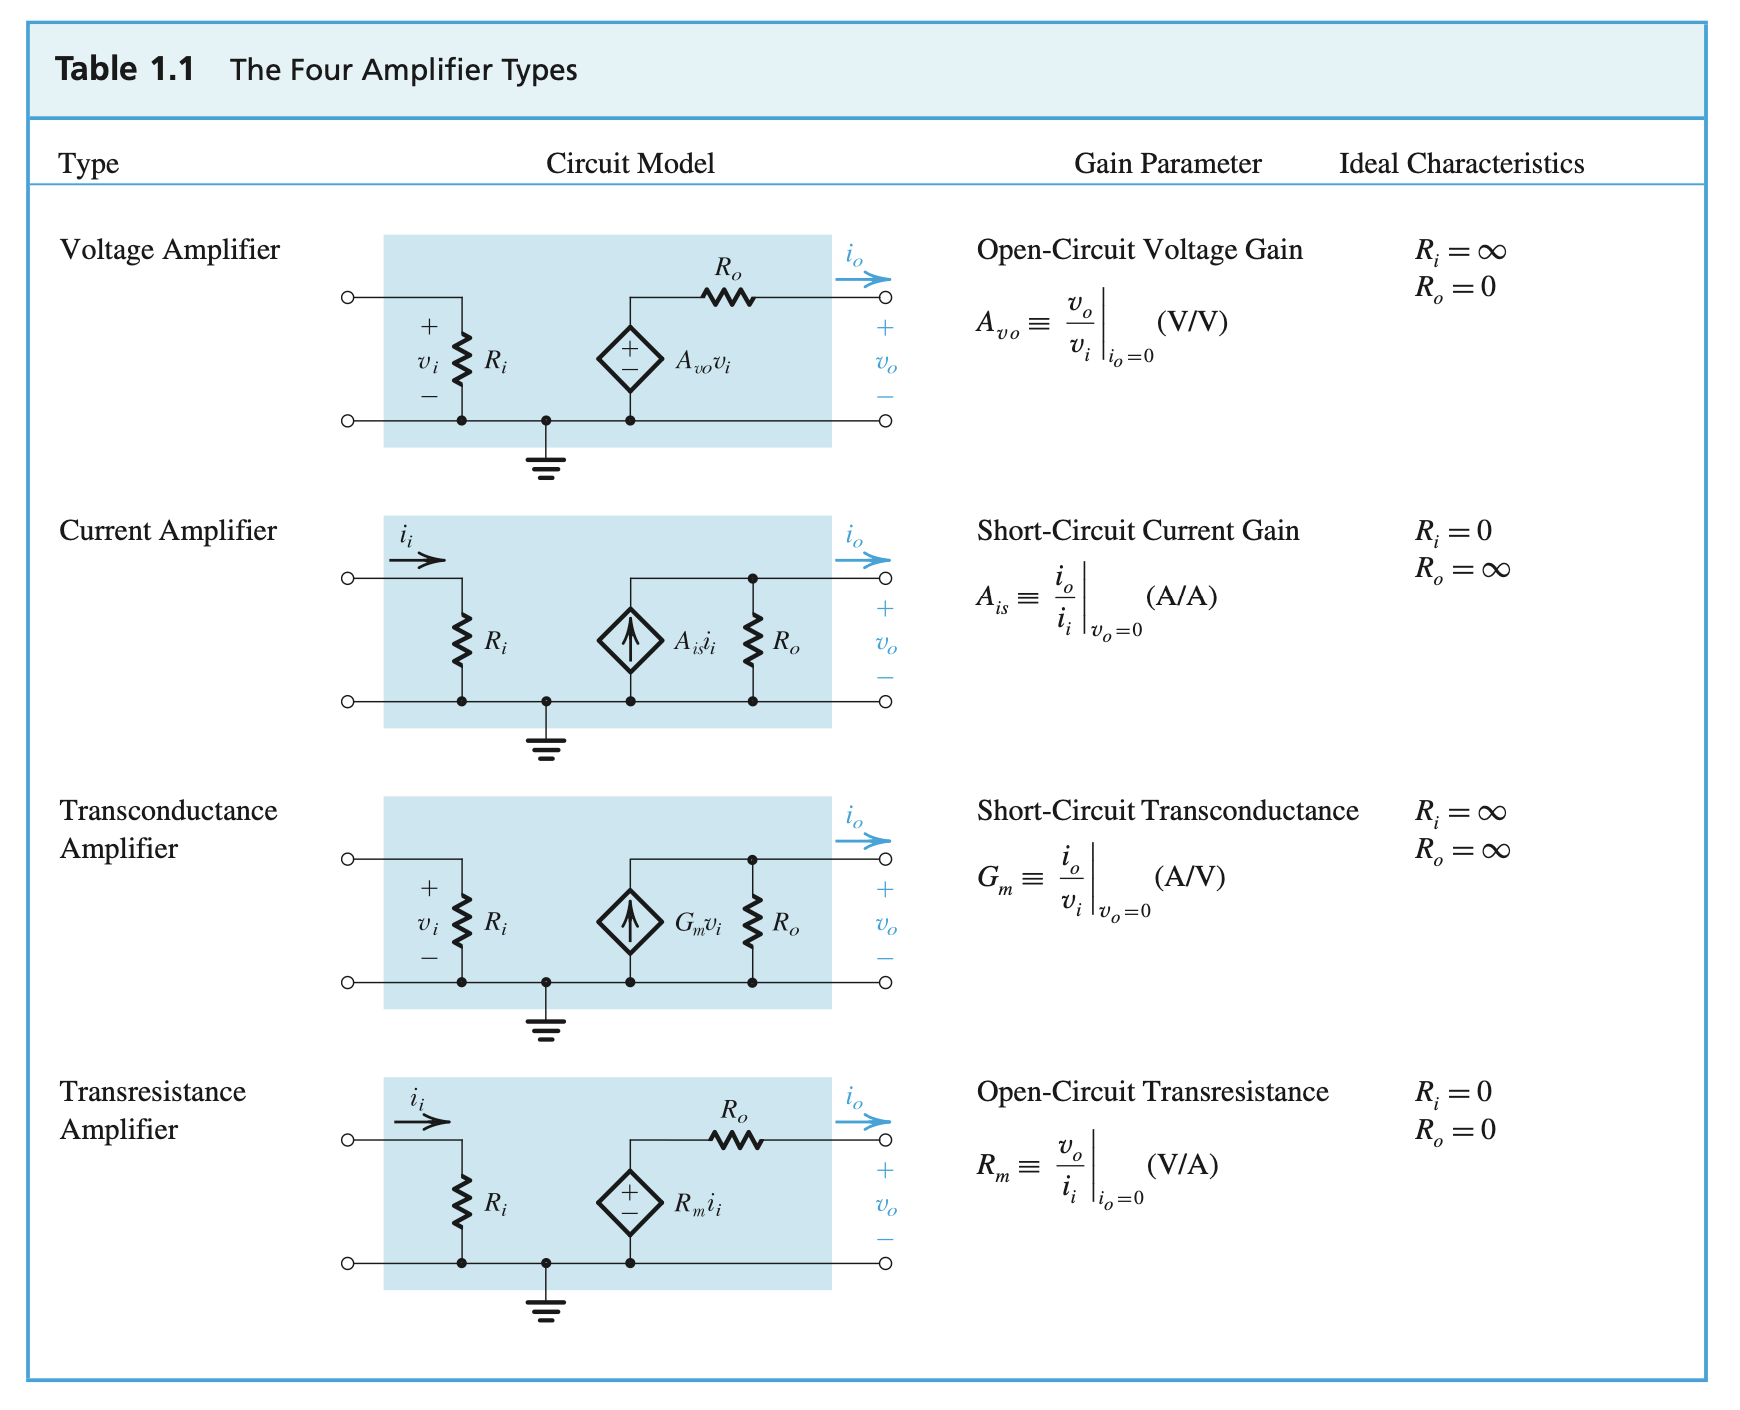
\includegraphics[scale=0.6]{figs/ch06/amplifier_types.png}
\end{figure}
In practice, there are other ways of finding input and output resistance, $R_i$ and $R_o$. You can find output resistance by measuring open-circuit output voltage to the short-circuit output current or by eliminating the input signal source and applying some voltage signal $v_x$ to the output of the amplifier. $R_o = v_x \slash i_x$. $i_x$ is the current frawn from $v_x$ into the output terminals. Input resistance can be found by measuring input current and input voltage.

If we ignore the body terminal of the MOSFET, we have a three terminal device. Since amplifiers is a four-terminal two-port, then this means that if we use two transistors one terminal must be common with each other. This leads to the following types of single stage amplifiers:
\begin{pline}
    \item Common source (CS) amplifier
    \item Common gate (CG) amplifier 
    \item Common drain (CD) amplifier
\end{pline}
BJT equivalents, respectively, are common emitter, common base, and common collector amplifiers. 

An inductor acts as an open circuit at high frequencies (remember by recalling its impedance, $j \omega L$ / $j 2 \pi f L$). We see that as we increase frequency, the impedance of the inductor increases as well. To summarize. an inductor at DC is a short-circuit and at AC is an open-circuit. The opposite is true for a capacitor. For this reason, infinitely large inductors, or \textbf{chokes}, are used in place of large resistors to isolate the \textit{DC supply or reference voltages} of sensitive circuits from the rest of the noisy system. 

AC coupling capacitors are ideally infinite and blocks DC, but allows AC to flow through.

\section{Common Source Amplifier}
Has the following parameters:
\begin{pline}
    \item Can develop gain
    \item High input impedance
    \item Inverting
\end{pline}

\section{Common Gate Amplifier}
A common gate amplifier has a current gain of unity, so it acts as a \textbf{currentÍ3‹ buffer}. It must meet the following requirements:
\begin{pline}
    \item Must have a current gain of unity
    \item Should present a low input impedance
    \item Should present a high output impedance
\end{pline}

\section{Common Drain Amplifier}
The signal input comes into the gate and the signal output leaves through the source and the drain is not grounded here and is instead connected to a DC voltage. Typically used as a \textbf{voltage buffer}.

\begin{todo}
    \item Insert into appropriate section
\end{todo}

\section{Practice Problems}

\begin{enumerate}
    \item Assume that the following circuits have the same large signal operating points and that $V_{tn}$ = 1V (without body bias), $k-n = \frac{\mu C_{ox} W}{L} = 10^{-3}$ A/V\sq, $\lambda = 0$, $\gamma = 0.5$ V$^{1/2}$, and $\phi_p = $ \SI{-400}{\milli \V}. $C_{big}$ means that the AC-coupling capacitor is so large that the lower bandwidth it imposes is far below any signal we are interested in and we can treat it as a short circuit for small-signal calculations (while still keeping it an open circuit for DC biasing calculations).
    \begin{todo}
        \item do this diagram is latex when you get the chance
    \end{todo}
    
    \begin{enumerate}
        \item What amplifier configurations are circuits
    \end{enumerate}
\end{enumerate}

\section{Sources}
\begin{itemize}
    \item EE105 Lecture 4/9/2024 by Alp Sipihigal
\end{itemize}